\chapter{加速器详细设计}\label{chap:accelerator}

本章分两个部分对加速器的设计过程进行说明,第一部分说明了 SIMD 架构的加速器设计的详细过程,第二部分说明了加速器的优化思路及优化过程。

\section{SIMD 架构的卷积神经网络加速器设计}

% 从对 YOLO V2 算法分析中可知,YOLO V2 算法除了路由层之外,其余各层都是将其上一层的输出作为下一层的输入,各层之间串行顺序处理。路由层的任务可以由设置存取地址的偏移实现,CNN 加速器只需要按照算法的流程,从内存对应地址读取数据,在加速器中进行运算,再将结果数据写入内存对应的地址即可。

从对 Darknet 的网络结构分析可知,YOLO V2 算法除了数据输入层之外,各层都是将上一层的输出数据作为本层的输入数据,层间的数据关联性较大,需要串行处理,而层内的数据关联性较小,可以使用 FPGA 进行并行加速。本文设计的加速器运行过程如图~\ref{fig:AcceleratorFlow}所示,CNN 加速器每次从 DDR 内存中读取多块数据写入缓存,CNN 加速器内部的运算单元从缓存获取数据,根据相应的配置参数进行判断,将数据分别交给 CONV、POLL、REORG 模块进行运算,运算的结果数据写入 CNN 加速器的缓存中,最后 CNN 加速器再将计算结果写回 DDR 内存中,由此完成了一整个计算流程。

\begin{figure}[!htbp]
    \centering
    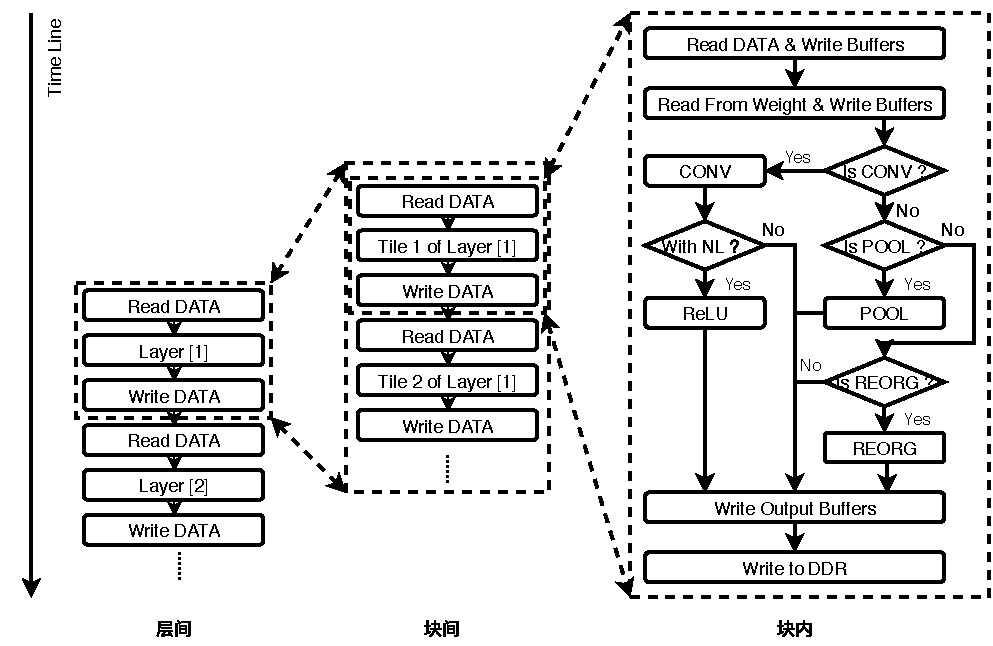
\includegraphics[width=0.9\textwidth]{AcceleratorFlow}
    \caption{CNN 加速器运行流程}
    \label{fig:AcceleratorFlow}
\end{figure}

% 整个加速器运行的流程如图~\ref{fig:AcceleratorFlow}所示,CNN 加速器每次从 DDR 内存中读取多块数据写入缓存,CNN 加速器内部的运算单元从缓存获取数据,根据相应的配置参数进行判断,将数据分别交给 CONV、POLL、REORG 模块进行运算,运算的结果数据写入 CNN 加速器的缓存中,最后 CNN 加速器再将计算结果写回 DDR 内存中,由此完成了一整个计算流程。

CNN 加速器结构如图~\ref{fig:AcceleratorStructure}所示,包含一个 AXI Lite 接口,以及 N 个 AXI Full 接口。其中,AXI Lite 连接在 RISC-V 处理器上,通过此接口,RISC-V 处理器可以对其进行功能的控制,选择 CNN 加速器的计算单元;一个 AXI Full 接口连接在 DDR 内存上,用于获取权重参数;另外的 N-1 个 AXI Full 连接在 DDR 内存上,用来写入或者读取特征图数据。CNN 加速器内部有四个计算单元,分别是 CONV、POLL、REORG 和 ReLU,这四个模块从 CNN 加速器的缓存中获取数据,通过 CNN 加速器中的寄存器控制,分别完成卷积、池化、重排序和激活的计算任务。Data Gather 模块负责生成数据读取地址,并且控制 AXI Full 接口从 DDR 内存中获取数据,将其写入 Input Buffer 模块中进行缓存。Data Scatter 模块负责生成写回地址,并且控制 AXI Full 接口,将 Output Buffer 中的数据写回 DDR 内存中。Weight Buffer 模块缓存负责权重数据。

\begin{figure}[!htbp]
    \centering
    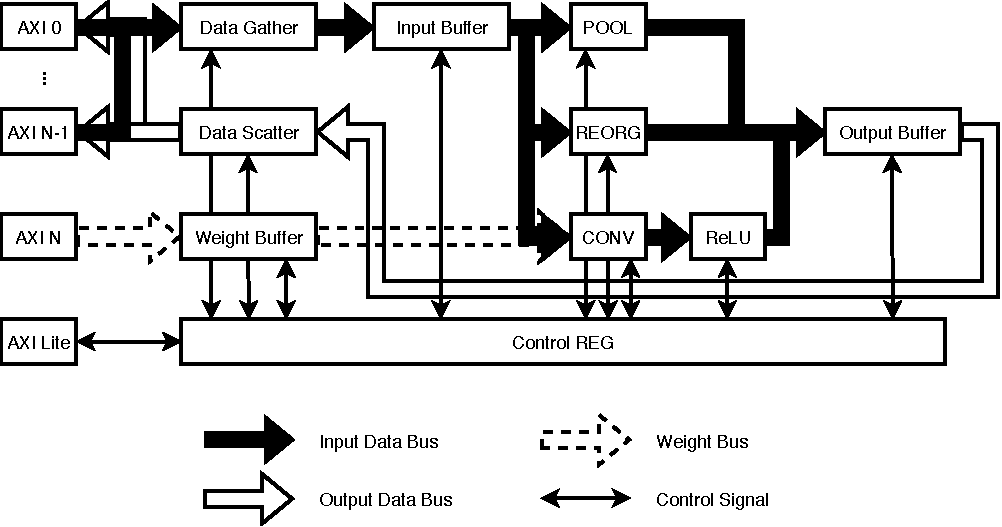
\includegraphics[width=0.9\textwidth]{AcceleratorStructure}
    \caption{CNN 加速器结构}
    \label{fig:AcceleratorStructure}
\end{figure}

负责读写特征图数据的 AXI Full 接口总数量可以由公式~\ref{eq:AxiNum}计算获得:
\begin{equation} \label{eq:AxiNum}
N_{Channel} = Max(N_{in}, N_{out})
\end{equation}

其中 $N_{Channel}$ 表示总的负责读写特征图数据的 AXI Full 接口数量,$N_{in}$ 表示读取特征图需要的 AXI Full 接口的数量,$N_{out}$ 表示输出特征图数据需要的 AXI Full 接口数量。由于 AXI Full 协议是一种全双工的总线协议,所以一条总线上读写操作可以同时进行,互不影响,所以实际上负责读写特征图数据的 AXI Full 接口总数量由读通道和写通道中多的一方决定。

\subsection{数据输入输出模块}

数据输入模块的硬件架构如图~\ref{fig:Input} 所示,Data Scatter 模块从 DDR 内存中获取 $Tif$ 张 $Tix \times Tiy$ 大小的特征图数据,然后依次分发到 CNN 加速器的 $Tif$ 个缓存模块中。数据输出模块的硬件架构如图~\ref{fig:Output} 所示,Data Gather 模块将 CNN 加速器中 $Tof$ 个缓存模块中的数据依次写入到 DDR 内存中。

\begin{figure}[!htbp]
    \centering
    \begin{subfigure}[b]{0.6\textwidth}
        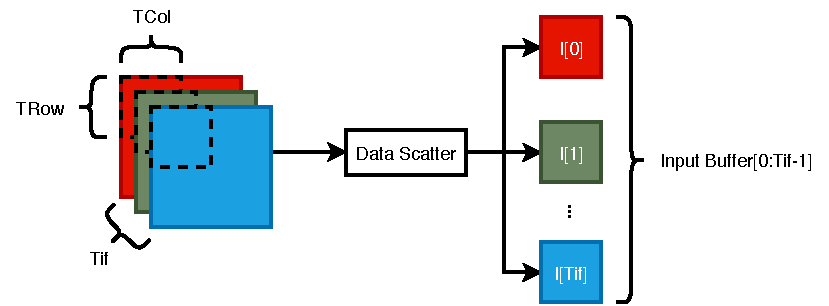
\includegraphics[width=\textwidth]{Input}
        \caption{数据输入模块}
        \label{fig:Input}
    \end{subfigure}
    \\% add desired spacing
    \begin{subfigure}[b]{0.6\textwidth}
        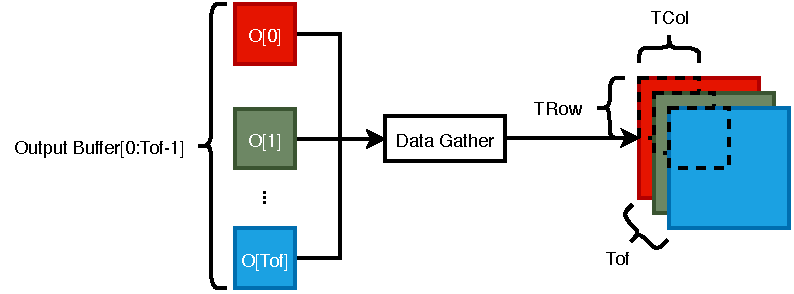
\includegraphics[width=\textwidth]{Output}
        \caption{数据输出模块}
        \label{fig:Output}
    \end{subfigure}
    \caption{数据输入输出模块硬件架构}
\end{figure}

为了保证数据的读写效率,使数据的输入输出部分不至于成为整个加速器的瓶颈,数据输入输出模块中使用双缓存的方案交替读取或者写入数据。

\begin{figure}[!htbp]
    \centering
    \begin{subfigure}[b]{0.6\textwidth}
        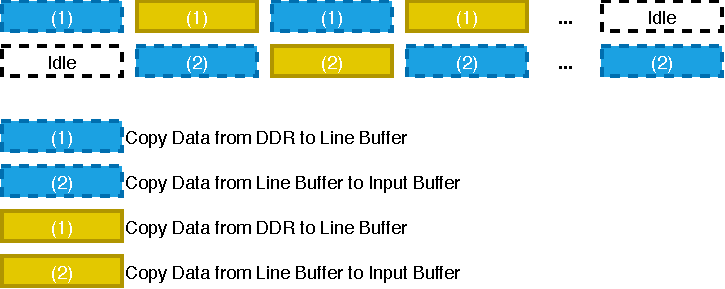
\includegraphics[width=\textwidth]{InputTime}
        \caption{数据输入模块时序}
        \label{fig:InputTime}
    \end{subfigure}
    \\% add desired spacing
    \begin{subfigure}[b]{0.6\textwidth}
        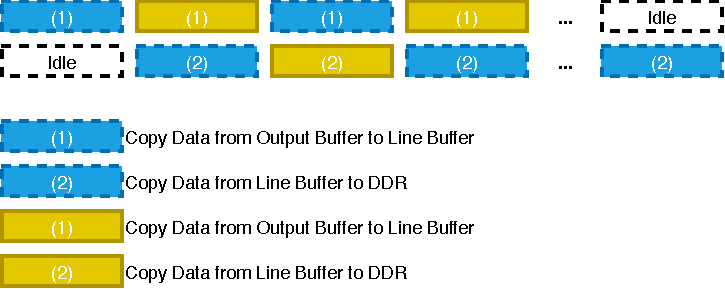
\includegraphics[width=\textwidth]{OutputTime}
        \caption{数据输出模块时序}
        \label{fig:OutputTime}
    \end{subfigure}
    \caption{数据输入输出模块双缓存时序}
\end{figure}

数据输入模块的时序如图~\ref{fig:InputTime} 所示,在流水线中,两个缓存模块交替完成从 DDR 内存中读取数据和将数据分发到 CNN 加速器内部的 Input Buffer 上的任务,考虑到数据读取和数据分发所产生的时延是相同的,因此在理想情况下,使用双缓存模式后,数据输入模块产生的时延仅为原先单缓存模式下的 $\frac{1}{2}$。

数据输出模块的时序如图~\ref{fig:OutputTime} 所示,在流水线中,两个缓存模块交替完成从 CNN 加速器内的 Output Buffer 上获取数据和将数据写入 DDR 内存的任务。和数据输入模块的时序相似,在理想情况下,使用双缓存模式后,数据输出模块产生的时延仅为原先单缓存模式下的 $\frac{1}{2}$。

\subsection{CONV 卷积模块}

由于卷积层有大量的乘加运算,占据了整个 CNN 计算的大部分时间,因此在硬件加速中,本设计将卷积层进行不同维度的展开,通过设计相应的并行乘加运算单元,来达到加速卷积计算的效果。基本的维度展开主要分以下 4 种:

\subsubsection{卷积核维度的展开}

\begin{figure}[!htbp]
    \centering
    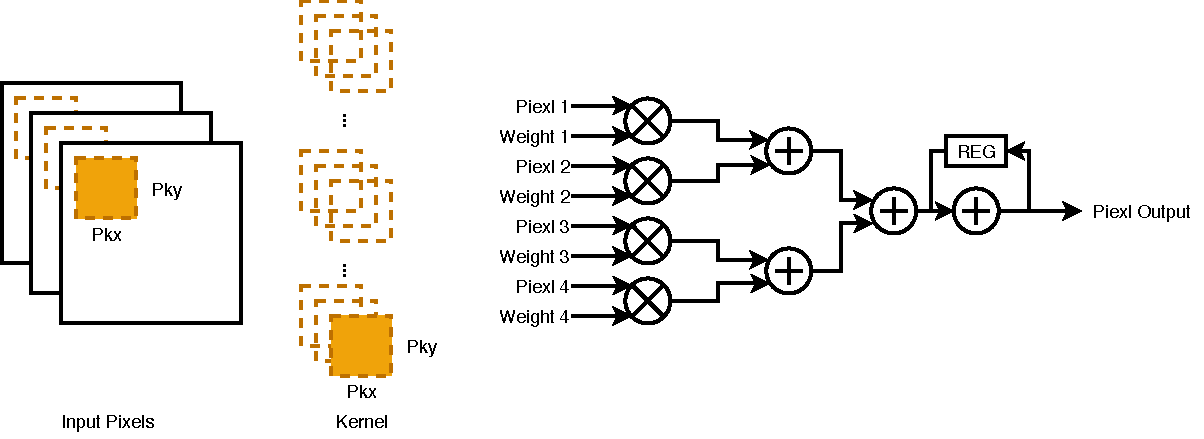
\includegraphics[width=0.8\textwidth]{UnfoldKernel}
    \caption{卷积核维度展开硬件架构}
    \label{fig:UnfoldKernel}
\end{figure}

如图~\ref{fig:UnfoldKernel}所示,展开卷积核的宽度 $Pkx$ 和卷积核的高度 $Pky$。在每个时钟周期里,同一输入特征图的相邻的 $Pkx \times Pky$ 个相邻的像素与卷积核对应位置的权重数据进行并行的乘法运算,乘法运算的结果通过一个深度为 $log_2{Pkx \times Pky}$ 的加法树相加得到中间结果,累加的结果存放在一个寄存器中。该维度展开卷积运算,消耗的资源为 $Pkx \times Pky$ 个乘法器、一个深度为 $log_2{Pkx \times Pky}$ 的加法树和一个累加器。

\subsubsection{输入特征图数维度的展开}

\begin{figure}[!htbp]
    \centering
    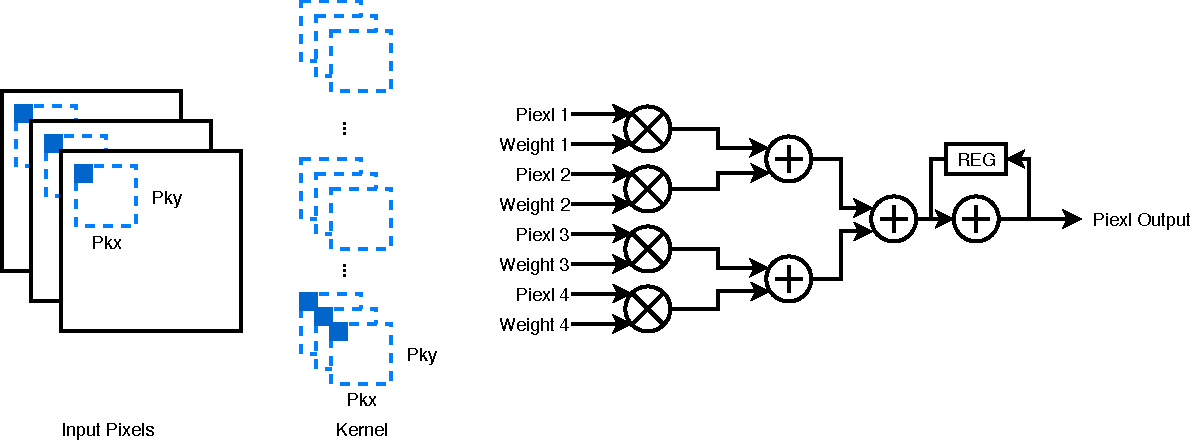
\includegraphics[width=0.8\textwidth]{UnfoldInput}
    \caption{输入特征图数维度展开硬件架构}
    \label{fig:UnfoldInput}
\end{figure}

如图~\ref{fig:UnfoldInput}所示,展开 $Pif$ 个输入特征图。在每个时钟周期里,同时从 $Pif$ 个输入特征图的同一位置读取一个像素与卷积核对应位置的权重数据进行乘法运算,乘法运算的结果通过一个深度为 $log_2{Pif}$ 的加法树相加得到中间结果,累加的结果存放在一个寄存器中。该维度展开卷积运算,消耗的资源为 $Pif$ 个乘法器、一个深度为 $log_2{Pif}$ 的加法树和一个累加器。

\subsubsection{输出特征图维度的展开}

\begin{figure}[!htbp]
    \centering
    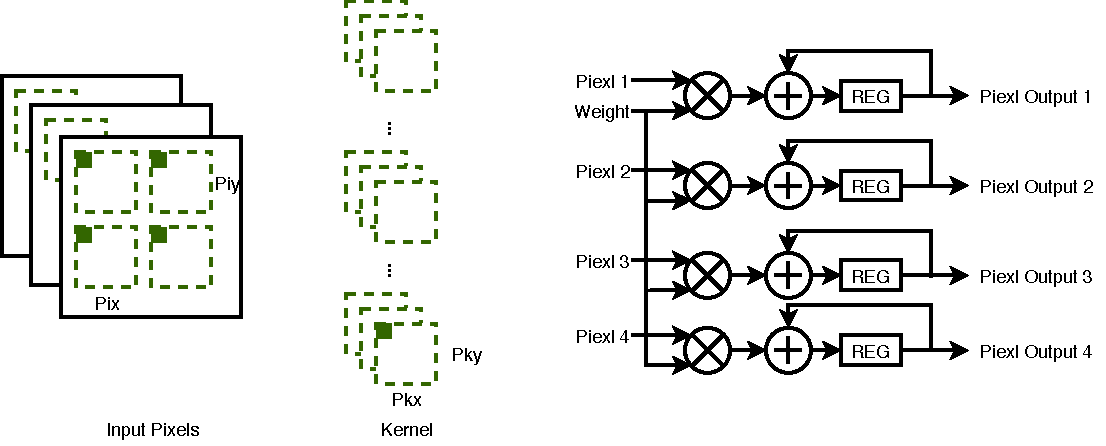
\includegraphics[width=0.8\textwidth]{UnfoldOutput}
    \caption{输出特征图维度展开硬件架构}
    \label{fig:UnfoldOutput}
\end{figure}

如图~\ref{fig:UnfoldOutput}所示,展开输出特征图的宽度 $Pix$ 和卷积核的高度 $Piy$。在每个时钟周期里,计算同一输出特征图的相邻的 $Pix \times Piy$ 个相邻的像素的值。该过程与卷积核维度的展开的运算类似。

\subsubsection{输出特征图数维度的展开}

\begin{figure}[!htbp]
    \centering
    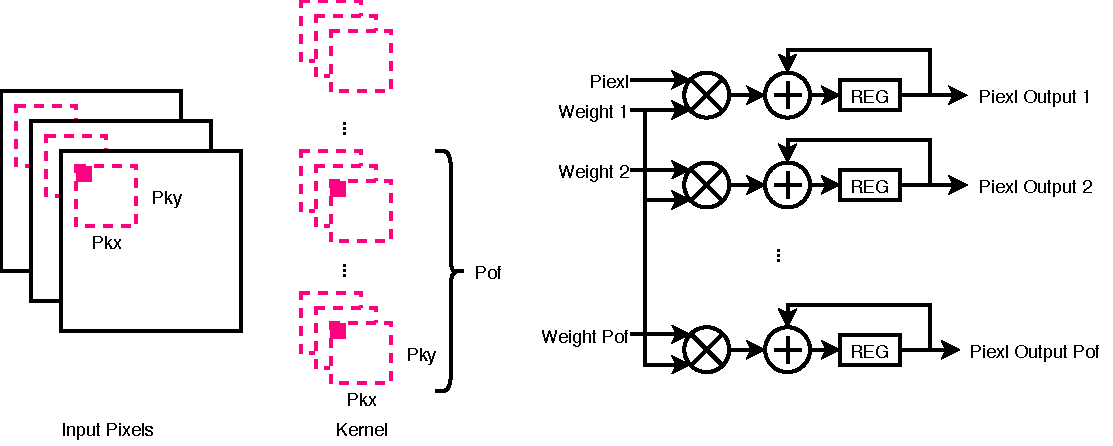
\includegraphics[width=0.8\textwidth]{UnfoldOutputNum}
    \caption{输出特征图数维度展开硬件架构}
    \label{fig:UnfoldOutputNum}
\end{figure}

如图~\ref{fig:UnfoldOutputNum}所示,展开 $Pof$ 个输出特征图。在每个时钟周期里,同时将同一个输入特征图的一个像素与 $Pof$ 个卷积核对应位置的权重数据进行乘法运算,乘法运算的结果通过一个深度为 $log_2{Pof}$ 的加法树相加得到中间结果,累加的结果存放在一个寄存器中。该维度展开卷积运算,消耗的资源为 $Pof$ 个乘法器、一个深度为 $log_2{Pof}$ 的加法树和一个累加器。

\subsubsection{卷积展开设计}

由于在 FPGA 中,图像数据是以数据流的形式进行传输的,即在流水线中,每个时钟周期传输一个像素的数据,如果想一个时钟周期同时访问 $N$ 个像素的数据,就需要 $N$ 条数据总线。但由于在本设计中,特征图数据是存储在外置的 DDR 中的,同时访问 $N$ 个像素的数据违背了 DDR 的工作原理,因此任然需要排队等待。所以这种需要同时访问多个像素数据的优化方式在访存部分会形成瓶颈,无法达到有效的加速效果。而展开方法(1)卷积核维度的展开与展开方法(3)输出特征图维度的展开正是有这种多个像素同时读取的需求,因此在本设计中使用的卷积展开方法主要是展开方法(2)输入特征图数维度的展开与展开方法(4)输出特征图数维度展开的结合使用。

\begin{figure}[!htbp]
    \centering
    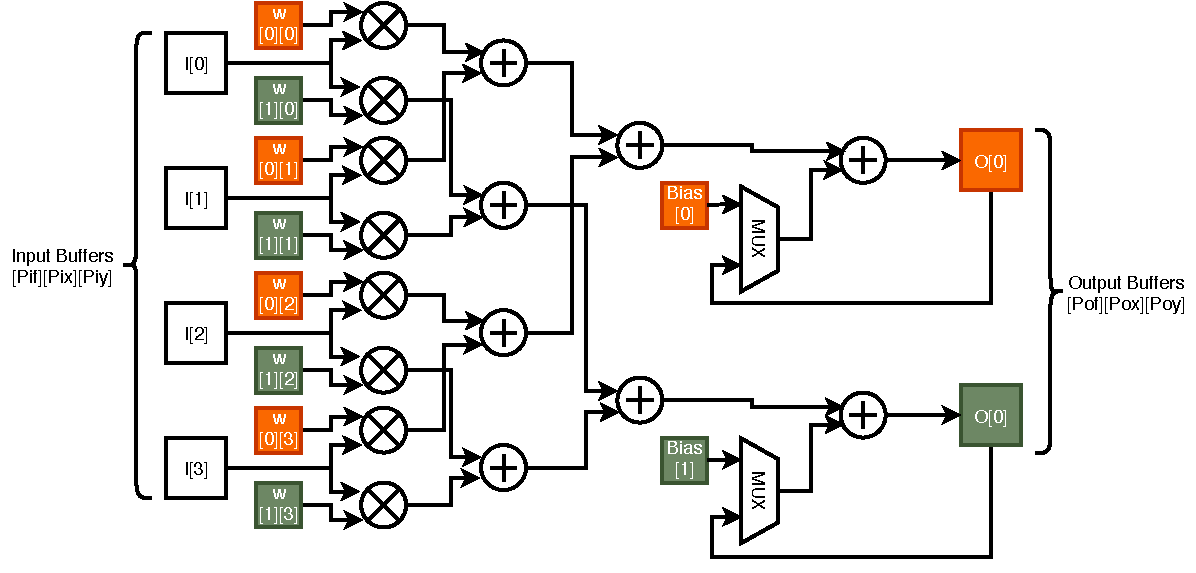
\includegraphics[width=0.8\textwidth]{Unfold}
    \caption{卷积模块硬件架构}
    \label{fig:Unfold}
\end{figure}

如图~\ref{fig:Unfold}所示,通过对输入特征图数维度于输出特征图数维度进行二维展开。以输入特征图数 $Pif = 4$ 和输出特征图数 $Pof = 2$ 为例,展开度为 $Pif \times Pof = 8$。在一个时钟周期内,同时从 $Pif$ 个输入特征图的同一位置读取一个像素分别和 $Pof$ 个卷积核对应的权重数据相乘,再将乘法的结果通过一个深度为 $log_2{Pif\times Pof}$ 的加法树相加,加法树输出的结果在通过一个累加器将局部运算的结果进行累加,最终的结果存放在 CNN 加速器的寄存器中。该展开方式消耗 $Pif \times Pof$ 个乘法器,一个深度为 $log_2{Pif \times Pof}$ 的加法树和一个累加器。

在内存访问速度不是瓶颈的情况下,即每个时钟周期可以获得一个输入特征图的像素,该展开方式进行卷积计算产生的时延如公式~\ref{eq:convlatency}所示。式中 $Latency_{CONV}$ 为一层卷积计算的总时延;$Const_{CONV}$ 为一个常量,代表了数据充满流水线所需要的时间;$Nky$ 与 $Nkx$ 分别表示输入特征图的高度和宽度;$Toy$ 和 $Tox$ 表示卷积核的高度和宽度。 
\begin{equation} \label{eq:convlatency}
Latency_{CONV} = (Const_{CONV} + Nky \times Nkx \times Toy \times Tox)/Freq
\end{equation}

可以看到,在该展开方式下,卷积运算的总时延与单层输入特征图,单层输出特征图的时延相当。因此在该展开方式下,卷积计算的总时延仅为原本的 $\frac{1}{Pof \times Pif}$,因此该展开方式可以有效的对卷积运算进行加速。

\subsection{POOL 池化模块}

由于图像中相邻位置的像素有着相似的值,卷积层的输出特征图同样也会在相邻区域有值相似的像素,因此去除这些相似值的像素并不会使特征图损失很多信息,并且通过去除这些相似的像素可以极大的减少参数数量,从而降低后续卷积运算的计算量,池化层就是完成了这个任务。池化运算与卷积运算类似,YOLO V2 算法中所有的池化层都是大小为 $2 \times 2$,步长 $S = 2$ 的最大池化。因此池化加速模块的设计可以参考卷积模块的设计,不同的是池化模块只需要对单一的输入特征图进行运算,并且运算单元由原先卷积模块中的乘加运算单元换成了比较运算单元。

\begin{figure}[!htbp]
    \centering
    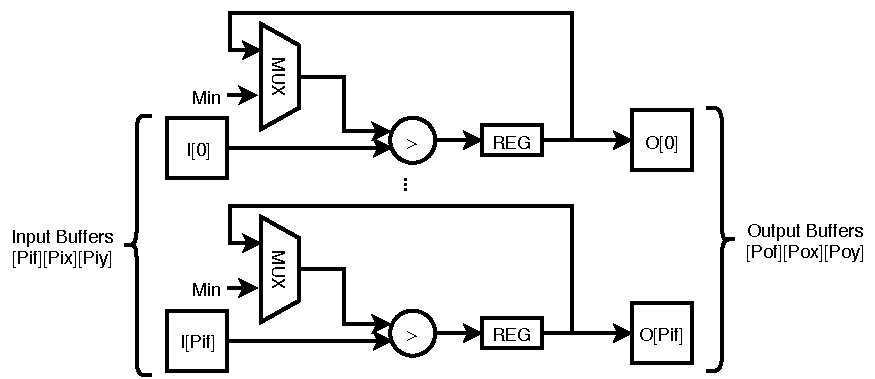
\includegraphics[width=0.80\textwidth]{pool}
    \caption{池化模块硬件架构}
    \label{fig:pool}
\end{figure}

如图~\ref{fig:pool} 所示,池化模块在运算过程中,同时从 $Pif$ 个输入特征图的同一位置获取一个像素,并与当前的最大值进行比较,在比较完成后,将得到的最大值写入输出缓存中。该结构的池化模块消耗 $Pif$ 个比较器和 $Pif$ 个寄存器。该池化运算加速模块的计算时延如公式~\ref{eq:pool}所示:
\begin{equation} \label{eq:pool}
Latency_{POOL} = (Const_{POOL} + Nky \times Nkx \times Toy \times Tox)/Freq
\end{equation}

式中 $Latency_{POOL}$ 为一层池化计算的总时延;$Const_{POOL}$ 为一个常量,代表了数据充满流水线所需要的时间;$Nky$ 与 $Nkx$ 分别表示输入特征图的高度和宽度;$Toy$ 和 $Tox$ 表示池化核的高度和宽度。 

\subsection{REORG 重排序模块}

重排序层的作用主要是对输入特征图进行一个拆分,将输入特征图相邻位置的像素分别输出到不同的特征图上。该过程的运算与池化模块的运算过程相似,不同的是池化模块将一个输入特征图输出到一个输出特征图,而重排序模块是将一个输入特征图输出到多个输出特征图。重排序模块的硬件架构如图~\ref{fig:reorg}所示。

\begin{figure}[!htbp]
    \centering
    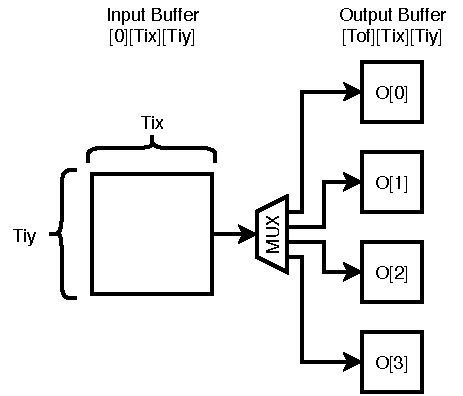
\includegraphics[width=0.40\textwidth]{reorg}
    \caption{重排序模块硬件架构}
    \label{fig:reorg}
\end{figure}

由于 YOLO V2 中的重排序层是 $Nky=Nkx=S=2$ 的结构,因此重排序层需要1个输入缓存模块和4个输出缓存模块,重排序模块的计算时延如公式~\ref{eq:reorg}所示:
\begin{equation} \label{eq:reorg}
Latency_{REORG} = (Const_{REORG} + Nky \times Nkx)/Freq
\end{equation}

式中 $Latency_{REORG}$ 为一层重排序计算的总时延;$Const_{REORG}$ 为一个常量,代表了数据充满流水线所需要的时间;$Nky$ 与 $Nkx$ 分别表示输入特征图的高度和宽度。

\section{CNN 加速器优化}

\subsection{乒乓缓冲优化}

乒乓缓冲在 FPGA 设计中是一种典型的以面积换时间的做法,在本次设计的 CNN 加速器中,我们在 CNN 加速器的数据输入端口和数据输出端口使用了乒乓缓冲的结构进行优化。因此该 CNN 加速器在流水线模式下运行时可以使数据传输产生的时延与数据运算产生的时延相重叠,加速器运算的总时延的计算如公式~\ref{eq:latency}所示:
\begin{equation} \label{eq:latency}
Latency_{ALL} = Max(Latency_{load},Latency_{compute},Latency_{store})
\end{equation}

式中 $Latency_{ALL}$、$Latency_{load}$、$Latency_{compute}$、$Latency_{store}$ 分别代表 CNN 加速器运算的总时延、从 DDR 内存中读取数据所产生的时延、加速器计算所产生的时延、将数据写回 DDR 内存中的所产生的时延。

\subsection{多数据通道传输优化}

由于 DDR 内存的带宽远大于一条 AXI4 总线的带宽,为了充分利用 DDR 内存的带宽,减少数据传输过程中产生的时延,在本设计中使用了多数据通道传输的优化方式。

\begin{figure}[!htbp]
    \centering
    \begin{subfigure}[b]{0.70\textwidth}
        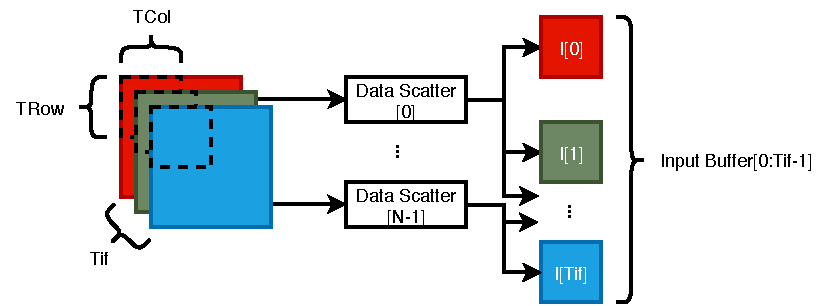
\includegraphics[width=\textwidth]{InputMult}
        \caption{数据输入模块}
        \label{fig:InputMult}
    \end{subfigure}
    \\% add desired spacing
    \begin{subfigure}[b]{0.70\textwidth}
        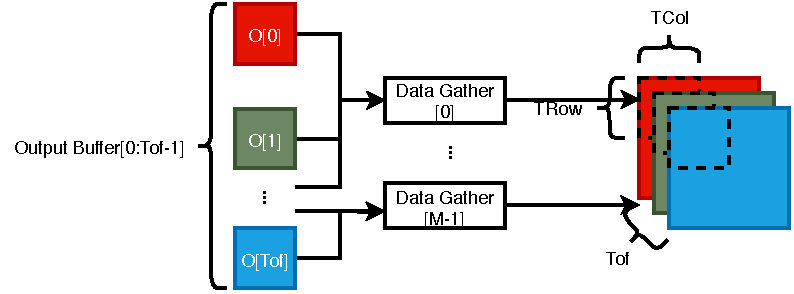
\includegraphics[width=\textwidth]{OutputMult}
        \caption{数据输出模块}
        \label{fig:OutputMult}
    \end{subfigure}
    \caption{多数据通道传输优化硬件架构}
\end{figure}

数据输入模块的多数据通道传输优化硬件架构如图~\ref{fig:InputMult} 所示,模块内部有多个独立的 Data Scatter 模块,每个模块有一条独立的 AXI4 总线,每个 Data Scatter 模块负责一部分数据缓存模块,因此多个 Data Scatter 模块可以并行地从 DDR 内存中读取特征图数据,并将数据分发到其负责的缓存模块上,从而提高了 DDR 内存的带宽利用率。

数据输出模块的多数据通道传输优化硬件架构如图~\ref{fig:OutputMult} 所示,与数据输入模块的优化思路相似,在模块内部使用多个独立的 Data Gather 模块,每个模块有一条独立的 AXI4 总线,因此多个 Data Gather 模块可以并行的将其负责的一部分缓存模块中的数据写入到 DDR 内存中 。

\section{本章小结}

本章对 CNN 加速器进行了详细的设计及优化。具体说明了四种卷积循环的展开模式以及各模式产生的时延和局限性,最终选取了输入特征图数维度的展开和输出特征图数维度的展开相结合的模式,从而在硬件资源的允许范围内,尽可能多的减少卷积运算产生的时延。同时由于硬件资源的限制,无法将 YOLO V2 模型的所有层同时进行硬件加速,因此采取了每次加速一层中一部分的做法,该方法类似于 FPGA 中状态机的思路,是一种用时间换面积的做法。由于该方法涉及大量的内存读写,为了使内存读写的时延不成为 CNN 加速器的瓶颈,加速器内部使用了双缓存和多数据通道的优化方法,保证了在流水线运行模式下,内存的读写时间可以被卷积运算的时间所掩盖,从而尽量减少内存的读写所产生的时延对加速器性能造成的影响。